\documentclass[journal]{IEEEtran}

\usepackage{cite}
\usepackage[]{algorithm2e}
\usepackage{color}
\usepackage{multirow}
\usepackage{subfigure}
\usepackage[justification=centering]{caption}
\usepackage{color}
\usepackage{graphicx}
\usepackage{float} 
\usepackage{epstopdf}


\usepackage[cmex10]{amsmath}
\usepackage{amsmath}
\usepackage{amssymb}
\usepackage[]{algorithm2e}
\usepackage{enumitem} 



%\hyphenation{op-tical net-works semi-conduc-tor}


\def\MK{\color{blue} {\bf Matthieu:} }



\begin{document}


\title{Structured Projective Non Negative Matrix Factorization with drum dictionaries for Harmonic/Percussive Source Separation}

\author{Cl\'{e}ment~Laroche,
        Matthieu~Kowalski,
        H\'{e}l\`{e}ne~Papadopoulos,~\IEEEmembership{Member,~IEEE,}
        and Ga\"{el}~Richard,~\IEEEmembership{Senior~Member,~IEEE}% <-this % stops a space
        
\thanks{This work was supported by a grant from DIGITEO}}



\maketitle


\begin{abstract}
In this paper, we propose a new unconstrained nonnegative matrix factorization method designed to use the multilayer structure of audio signals in order to improve the quality of source separation. Audio signals (and music signals in particular) can be decomposed in two distinct parts: a tonal component which is sparse in frequency and temporally stable and a transient component composed of short term broadband sounds. Our method decomposes the audio signal in sparse orthogonal components that are well suited for representing the tonal component, while the transient part is represented by a regular nonnegative matrix factorization decomposition. Experiments on a large database of real music data show that such decomposition is suitable for audio source separation. Tested in comparison with three state-of-the-art harmonic/percussive decomposition algorithms, the proposed method shows competitive performances.
\end{abstract}


\begin{IEEEkeywords}
nonnegative matrix factorization, projective nonnegative matrix factorization, audio source separation, harmonic/percussive decomposition.
\end{IEEEkeywords}


\section{Introduction}
\label{sec:intro}


Harmonic/percussive source separation (HPSS) is based on the observation that harmonic instruments are tonal sounds very localized in frequency that can be modeled by a sum of sinusoidal waves and percussive instruments are wide band transient signals.

Harmonic instruments can be classified into several categories such as for example struck string instruments (piano, harpsichord, \ldots), plucked string instruments (guitar, mandolin, \ldots) or brass instruments (trumpet, tuba, \ldots)~\cite{peeters2003automatic}. These instruments can be modeled as a sum of three components: the Sinusoidal part, the Transients and the Residual, so called  Sines + Transients + Noise (STN) models~\cite{daudet2006review}. The transient of the harmonic instruments show some percussive properties (i.e., fast attack and fast decay). Taking into account the transient part of harmonic instruments is a challenging task that will not be treated this article. Here, as in other article of the literature, we rely on the hypothesis that most of the energy of the harmonic signal is in the tonal part. 


HPSS has numerous applications as a preprocessing step. For example most multi-pitch estimation models~\cite{klapuri2008multipitch}, instruments recognition~\cite{eronen2000musical} and melody extraction~\cite{salamon2012melody} ISMIR RIGAUD algorithms are much more efficient on harmonic instruments alone. Indeed, these algorithms often rely on the analysis of the harmonic structures that are blurred by the percussive instruments. Similarly, drum transcription algorithms~\cite{paulus2005drum} CITE ISMIR are more accurate if the harmonic instruments are not part of the signal. Finally, using the Median Filtering (MF) algorithm~\cite{fitzgerald2010harmonic} as a preprocessing step increases the performance for singing pitch extraction and voice separation~\cite{hsu2012tandem}. 


A well known unsupervised method to extract the harmonic/percussive components consists in applying a Median Filtering (MF) on the spectrogram of the audio signal~\cite{fitzgerald2010harmonic}. The filtering is made across the temporal atoms to diminish the transient sounds in order to extract the harmonic components. Mutually, the filtering is made across frequency to reduce the harmonic tonal sounds and to enhance the percussive instruments. The assumption made is that the harmonics are considered to be outliers in a temporal frame that contains a mixture of percussive and pitched instruments. Similarly, the percussive onsets are considered to be outliers in a frequency frame. This method is often used in the \emph{Music Information Retrieval} community as it does not require any parameter tuning and is computationally effective. The main problem of this method is that it does perform well on non stationary signal and the voice for example is spliced between the harmonic and percussive part. 
% However, on a small scale test conducted by~\cite{canadas2014percussive}, this simple approach does not give the best separation results.

Another unsupervised method uses a NMF decomposition with specific constraints to distinguish the harmonic part from the percussive components~\cite{canadas2014percussive}. A simple approximation is that percussive instruments are transient sounds with regular spectra (wide band signals) whereas harmonic instruments are tonal sounds with harmonic sparse spectra. This method gives good results compared to other state-of-the-art methods but this article will show that the results depend heavily on the training database.

A supervised method uses a Non-Negative Matrix Partial Co-Factorization (NMPCF)~\cite{kim2011nonnegative} to extract the drums. The spectrogram of the signal and the drum-only data (obtained from prior learning) are simultaneously decomposed in order to determine common basis vectors that capture the spectral and temporal characteristics of drum sources. The shared dictionary matrix retrieves the drum signal. However it must be chosen carefully in order to obtain satisfying results. The percussive part of the decomposition is constrained while the harmonic part is completely unconstrained. As a result, it tends to decompose a lot of information (i.e., the harmonic part contains some percussive instruments) from the signal and the decomposition is not satisfactory.
% In the NMPCF, the dictionary is not fixed. We will compare this method to the SPNMF were the dictionary is fixed. 

%This has motivated the development of methods for HPSS in the music signal processing area. We will focus on three methods that are particularly relevant to our benchmark. 

%Finally some methods use a so-called semi-supervised algorithm where data from scores helps the constrained decomposition method~\cite{hennequin2011score,fritsch2013score} %{\MK Je pense que ce paragraphe peut √™tre supprim√©: il n'en dit pas assez, et je ne suis pas s√ªr qu'il soit n√©cessaire de d√©velopper. Ou alors, il faut l'int√©grer au paragraphe suivant qui parle de technique semi-supervis√©e. Mais la, il me parait un peu esseul\'e.} {\HP OK pour l'intégrer à la suite. Definir méthode semi-supervisee, citer comme exemple celles [15,16] et dire pourquoi celle proposée rentre dans cette categorie.}


In this article, we propose a weakly-supervised decomposition technique suitable for harmonic/percussive source separation of non vocal monophonic instrumental signals. The sparse and orthogonal components of the Projective NMF (PNMF) are prone to extract the harmonic instruments well localized in frequency, while the percussive part with flat spectra are extracted by the NMF components. However, as shown in~\cite{laroche2015structured} this approach obtains limited performances in a blind source separation task when the percussive part is unconstrained. To force the non-orthogonal components to extract the drum signal, we use a dictionary specific to drum signals using the same technique as in~\cite{wudrum}.

The contributions of this article are threefold
\begin{enumerate}
\item The Structured Projected Nonnegative Matrix Factorization (SPNMF) method is introduced, as well as a simple multiplicative algorithm to solve the SPNMF problem.
\item  We offer a comparison between two different training methods to establish the best drum dictionary.
\item We perform a benchmark against three state of the art harmonic/percussive methods on a large database.	
\end{enumerate}

%}

The paper is organized as follows. In Section~\ref{sec:Background}, we describe the problem of harmonic/percussive source separation and we explain in details some recent state-of-the-art methods. The proposed SPNMF is then introduced in Section~\ref{sec:SPNMF}. We present our experimental protocol and the results obtained on synthetic and real audio signals in Section~\ref{sec:experiments}. Section~\ref{sec:stateoftheart} is a benchmark with state of the art methods. Finally, some conclusions are drawn in Section~\ref{sec:conc}.




\section{Context of harmonic/percussive decomposition}
\label{sec:Background}

%{\HP Introduire les deux classes d'instruments (harmonic/percussive) avant de détailler les instruments harmoniques.}
Harmonic/percussive source separation is based on the observation that harmonic instruments are tonal sounds very localized in frequency that can be modeled by sum of sinusoidal waves and percussive instruments are wide band transient signals.

Harmonic instruments can be classified into several categories such as for example struck string instruments (piano, harpsichord, \ldots), plucked string instruments (guitar, mandolin, \ldots) or brass instruments (trumpet, tuba, \ldots) \cite{peeters2003automatic}. These instruments can be modeled as a sum of three components: the Sinusoidal part, the Transients and the Residual, so called  Sines + Transients + Noise (STN) models~\cite{daudet2006review}. The transient of the harmonic instruments show some percussive properties (i.e., fast attack and fast decay). Taking into account the transient part of harmonic instruments is a challenging task that will not be treated this article. Here, as in other article of the literature, we rely on the hypothesis that most of the energy of the harmonic signal is in the tonal part. 

Harmonic/percussive source separation has numerous applications as a preprocessing step. For example most multi-pitch estimation models~\cite{klapuri2008multipitch}, instruments recognition~\cite{eronen2000musical} and melody extraction~\cite{salamon2012melody} algorithms are much more efficient if the influence of the percussive sources is diminished. Indeed, these algorithms often rely on the analysis of the harmonic structures that are blurred by the percussive instruments. Similarly, beat tracking~\cite{ellis2007beat} and drum transcription algorithms~\cite{paulus2005drum} are more accurate if the harmonic instruments are not part of the signal. Finally, using the Harmonic/Percussive Source Separation (HPSS) algorithm~\cite{fitzgerald2010harmonic} as a preprocessing step increases the performance for singing pitch extraction and voice separation~\cite{hsu2012tandem}. This has motivated the development of methods for harmonic/percussive sound separation in the music signal processing area. Numerous other methods exist but in this work, we will focus on three other methods that are particularly relevant to our benchmark. 

%{\HP This has motivated the development of mettons for harmonic/percussive sound separation in the music signal processing area. \bold{remarque: } Il y a de nombreuses approches pour l'HPSS qui existent mais seulement 3 sont choisies ici, et ce choix a l'air arbitraire. Il faut dire (en deux mots) qu'il y en a beaucoup d'approches (on peut par exemple une classification recente comme celle de l'article de Tachibana et al. de 2014 ``Harmonic/Percussive Sound Separation Based on Anisotropic Smoothness of Spectrograms''). Ensuite dire qu'on se concentre ici sur 3 methodes pour les raisons suivantes : \cite{ono2008separation} parce qu'elle est simple et populaire, \cite{canadas2014percussive} parce qu'elle est a l'oppose de celle qu'on présente, avec beaucoup d'hyperparametres et \cite{kim2011nonnegative} parce qu'il y a une similarite d'idee avec l'approche presentee. Bref, retravailler un peu cette deuxieme partie de la Section II.}

A well known unsupervised method to extract the harmonic/percussive components consists in applying a median filtering on the spectrogram of the audio signal~\cite{fitzgerald2010harmonic,ono2008separation}. The filtering is made along the temporal atoms to diminish the transient sounds in order to extract the harmonic components. Mutually, the filtering is made along the frequency to reduce the harmonic tonal sounds and to enhance the percussive instruments. The assumption made is that the harmonics are considered to be outliers in a temporal frame that contains a mixture of percussive and pitched instruments. Similarly, the percussive onsets are considered to be outliers in a frequency frame. This method is often used in the music information retrieval community as it does not require any parameter tuning and is computationally effective. However, on a small scale test conducted by~\cite{canadas2014percussive}, this simple approach does not give the best separation results.% {\HP dans quell contexte? par rapport à quoi? Quels signaux de test ? }.

Another unsupervised method uses a NMF decomposition with specific constraints to distinguish the harmonic part from the percussive components~\cite{canadas2014percussive}. A simple approximation is that percussive instruments are transient sounds with regular spectra (wide band signals) whereas harmonic instruments are tonal sounds with harmonic sparse spectra. From this observation, a frequency regularity and a temporal sparsity constraints are applied during the optimization process to extract the percussive instruments and vice-versa a temporal regularity and a frequency sparsity constraints are applied to extract the harmonic instruments. This method gives good results compared to other state-of-the-art methods~\cite{canadas2014percussive} but the hyper-parameters tuning is a tedious process and results depend heavily on the training database.

Finally in~\cite{kim2011nonnegative}. The drum source separation is done using a Non-Negative Matrix Partial Co-Factorization (NMPCF). The spectrogram of the signal and the drum-only data (obtained from prior learning) are simultaneously decomposed in order to determine common basis vectors that capture the spectral and temporal characteristics of drum sources. The shared dictionary matrix retrieves the drum signal, however it must be chosen carefully in order to obtain satisfying results. The percussive part of the decomposition is constrained while the harmonic part is completely unconstrained. As a result, it tends to decompose a lot of information (i.e., the harmonic part contains some percussive instruments) from the signal and the decomposition is not satisfactory. In the NMPCF, the dictionary are not fixed, we will this method compare it to the SPNMF were the dictionary is fixed. 


\section{Structured projective NMF (SPNMF)}
\label{sec:SPNMF}

In this section we present our semi-supervised algorithm for harmonic/percussive source separation.

\subsection{Principle of the SPNMF}

The orthogonal basis functions of the PNMF are not flexible enough to decompose a complex audio signal. As stated in~\cite{canadas2014percussive}, harmonic instruments have sparse basis functions whereas percussive instruments have much flatter spectra. As the columns of $W$ are orthogonal, when two sources overlap in the Time-Frequency (TF) plane only one basis function will represent the mixture which is not adequate for efficient separation. To overcome this problem, we propose to add a standard NMF decomposition term to the PNMF. We can expect that most of the harmonic components will be represented by the orthogonal part while the percussive ones will be the regular NMF components. Using a similar model to preliminary work~\cite{laroche2015structured}, let $V$ be the magnitude spectrogram of the input data. The model is then given by
\begin{equation} \label{Cfunction}
V \approx \tilde{V}= V_H + V_{P},
\end{equation}
with $V_P$ the spectrogram of the percussive part and $V_H$ the spectrogram of the harmonic part. $V_H$ is approximated by the PNMF decomposition while $W_P$ is decomposed by some NMF components as :
\begin{equation}
V \approx \tilde{V}= W_{H}W_{H}^{T}V + W_{P} H_{P}.
\end{equation}
The data matrix is approximated by an almost orthogonal sparse part that codes the harmonic instruments $V_H = W_HW_H^T V$ and a non constrained NMF part that codes the percussive instruments $V_P = W_PH_P$. The main advantage of the SPNMF results is in the fact that the method has few parameters compared to constrained NMF~\cite{canadas2014percussive} and NMPCF~\cite{kim2011nonnegative} while still obtaining similar results~\cite{laroche2015structured}. 


\subsection{Using regularized NMF for the harmonic part}

In order to highlight the advantages of using the PNMF for the harmonic part, we also designed a regularized method. Let $V$ be the magnitude spectrogram of the input data, the model is given by 
\begin{equation}
V \approx \tilde{V} = W_HH_H + W_P  H_P.
\end{equation}
The optimization problem is then:
\begin{equation}\label{REGNMF}
\min_{W_{H},W_{P},H_{P}}D(V|\tilde{V}) + k_{TSM} TSM + k_{SSP} SSP.
\end{equation} 

The constraints TSM and SSP are from equation \eqref{TSM} and \eqref{TSM} respectively. The hyperparameters $k_{TSM}$ and $k_{SSP}$ control the amount of temporal smoothness and spectral sparseness. This model replace the PNMF components by a regularized NMF (RegNMF) to extract the harmonic part. This requires prior tuning of the variables $k_{SSP}$ and $k_{SSP}$. 


\subsection{Optimization Algorithm}

In order to achieve such a decomposition, we can use a measure of fit $D(x|y)$ between the data matrix $V$ and the estimated matrix $\tilde{V}$. $D(x|y)$ is a scalar cost function and in this article we compare in Section \ref{setup:divergence} the use of the Euclidean distance (Euc), the Kullback Leiber (KL) divergence and the Itakura Saito (IS) divergence which are three commonly used divergences in the NMF framework.



The SPNMF model gives the following cost function : 
\begin{equation}\label{InitCost}
\min_{W_H,W_P,H_P \geq 0} D(V|W_{H}W_{H}^{T}V + W_{P} H_{P})  
\end{equation}

A solution of this problem can be obtained by iterative multiplicative update rules following the same strategy as in~\cite{yuanOja2005,Lee01algorithmsfor} which consists in splitting the gradient with respect to (wrt) one variable (here $W_H$ for exemple) $\nabla_{W_H} D(V|\tilde{V})$ in its positive $[\nabla_{W_H} D(V|\tilde{V})]^{+}$ and negative parts $[\nabla_{W_H} D(V|\tilde{V})]^{-}$.
The multiplicative updates for SPNMF are then given by: 
$$W_{H} \leftarrow W_{H} \otimes \frac{ [\nabla_{W_H} D(V|\tilde{V})]^{-} }{[\nabla_{W_H} D(V|\tilde{V})]^{+}}, $$
where $\otimes$ is the Hadamard product or element-wise product. Details of the equations for the Euc distance, KL and IS divergences are given in the annex in Sections \ref{euclidisteq}, \ref{KLdisteq} and \ref{ISdisteq} respectively. 
The optimization of the SPNMF algorithm is done sequentially, as described in Algorithm \ref{AlgoMultipl}.

\begin{algorithm}[h]
 Input: $V \in \mathbb{R}_{+}^{m \times n} $
 Output: $W \in \mathbb{R}_{+}^{m \times k}$, $W_P \in \mathbb{R}_+^{m \times e}$ and $H_P \in \mathbb{R}_{+}^{e \times n}$
 Initialization\;
 \While{$i \leq$ number of iterations}{
	$W_{P} \leftarrow W_{P} \otimes \frac{ [\nabla_{W_P} D(V|\tilde{V})]^{-} }{[\nabla_{W_P} D(V|\tilde{V})]^{+}}$
	 \vspace{0.2cm}

	$H_{P} \leftarrow H_{P} \otimes \frac{ [\nabla_{H_P} D(V|\tilde{V})]^{-} }{[\nabla_{H_P} D(V|\tilde{V})]^{+}}$
	

	$W_{H} \leftarrow W_{H} \otimes \frac{ [\nabla_{W_H} D(V|\tilde{V})]^{-} }{[\nabla_{W_H} D(V|\tilde{V})]^{+}}$
	 \vspace{0.2cm}
	 	
	$i=i+1$ 
 }
 $ V_P = W_PH_P $ and
 $ V_H = W_HW_H^TV $ 
  
 \vspace{0.2cm}
 \caption{SPNMF algorithm with multiplicative update rules.}\label{AlgoMultipl}
\end{algorithm}


\subsection{SPNMF with a fixed dictionary}\label{fixedict}  

A fully unsupervised SPNMF model does not allow for a satisfying harmonic/percussive source separation~\cite{laroche2015structured}. To alleviate this problem, we use here a fixed drum dictionary $W_p$ for the percussive part of the SPNMF which is created using the drum database ENST-Drums~\cite{gillet2006enst}. In this database three professional drum players specialized in a specific type of music have been recorded. Each drummer used a specific drum set from a small one (two toms and two cymbals) to a full rock drum kit (four toms and five cymbals). 

%Two different ways can be used to build a dictionary. 
The main method to construct a dictionary is to perform a NMF decomposition on a large database~\cite{jaureguiberry2011adaptation}. The rank of factorization is an important learning variable that will be discussed in a later section. This method is effective at giving a dictionary specific to an instrument and the size of the dictionary is maintained low so it does not increase the computation time. However, the template of the dictionary does not represent a single element of the drum kit so it is not possible to perform direct drum transcription.

%A second way to build the dictionary is to directly use the STFT of a drum signal~\cite{wudrum}. The ENST-Drum database contains audio files where elements of the drum kit are played independently and that we used to build other types of drum dictionary. This method allows having a specific dictionary, yet the matrix is redundant and very large which increases the computation time. Both learning methods are compared in Section \ref{setup:dictionary}.

The main advantage of the proposed method over the previously mentioned concurrent approaches is that it can take into account some of the percussive instruments that have a sparse spectrum. The bass drum and the toms have almost harmonic spectra with most energy in the low frequency range. These sounds are consequently hard to extract while enforcing frequency regularity of the percussive part like in~\cite{canadas2014percussive,ono2008separation}.

The SPNMF algorithm with the fixed dictionary matrix is described by Algorithm \ref{AlgoDictionary}.
 
\begin{algorithm}[h]
 Input: $V \in \mathbb{R}_{+}^{m \times n} $
 Output: $W \in \mathbb{R}_{+}^{m \times k}$, $W_{train} \in \mathbb{R}_+^{m \times e}$ and $H \in \mathbb{R}_{+}^{e \times n}$
 Initialization\;
 \While{$i \leq$ number of iterations}{
	$H_{P} \leftarrow H_{P} \otimes \frac{ [\nabla_{H_P} D(V|\tilde{V})]^{-} }{[\nabla_{H_P} D(V|\tilde{V})]^{+}}$
	

	$W_{H} \leftarrow W_{H} \otimes \frac{ [\nabla_{W_H} D(V|\tilde{V})]^{-} }{[\nabla_{W_H} D(V|\tilde{V})]^{+}}$
	 \vspace{0.2cm}
	 	
	$i=i+1$ 
 }
 $ V_P = W_{train}H_P $ and
 $ V_H = W_HW_H^TV $ 
  
\vspace{0.2cm}
 \caption{SPNMF with the drum dictionary matrix.}\label{AlgoDictionary}
\end{algorithm}


 
 
\subsection{Signal reconstruction}

The percussive signal $x_p(t)$ is synthesized using the magnitude percussive spectrogram $V_P = W_PH_P$. To reconstruct the phase of the percussive part, we use a generalized Wiener filter~\cite{liutkus:hal-01110028} to create a percussive mask as:
\begin{equation}
\mathcal{M}_P = \frac{V_P^2}{V_M^2 + V_P^2},
\end{equation} 
\noindent, To retrieve the percussive signal as 
\begin{equation}
x_p(t) = InverseSTFT(\mathcal{M}_P \otimes X),
\end{equation}
\noindent where $X$ is the complex spectrogram of the mixture.

Similarly for the harmonic part, we obtain:
\begin{equation}\label{percuwiener}
\mathcal{M}_H = \frac{V_H^2}{V_M^2 + V_P^2},
\end{equation}
and:
\begin{equation}
x_h(t) = InverseSTFT(\mathcal{M}_H \otimes X).
\end{equation}




\section{Experimental Validation of SPNMF}
\label{sec:experiments}

In this section we conduct experiments to understand the behaviour of the proposed method. We first perform a test on a synthetic signal to validate the model of SPNMF in Section~\ref{SynthTest}. We then set-up the SPNMF to perform efficient source separation by quantifying the influence of the rank of factorization in Section~\ref{setup:rank}, the effect of different divergence in  Section~\ref{setup:divergence} and finally the performance of the separation with different types of dictionaries in  Section~\ref{setup:dictionary}.


\subsection{Synthetic Tests}\label{SynthTest}

To illustrate how the SPNMF works without dictionary, we use a simple synthetic signal. The test signal models a mix of harmonic and percussive instruments. The harmonic part is simulated by a sum of sine waves that overlap in time and frequency. The first signal simulates a $C(3)$ with fundamental frequency $f_0 = 131$~Hz, the other one a $B(4)$ with $f_0 = 492$~Hz. To simulate the percussive part, we add $0.1$~s of Gaussian white noise for the first two second. For the last two seconds, we add $0.3$~s of Gaussian white noise filtered by a high-pass filter. The signal is $5$~s long and the sampling rate is $4000$~Hz. We compute the Short Time Fourier Transform (STFT) with a $512$ sample-long ($0.128$~s) Hann analysis window and a $50\%$ overlap. The spectrogram of the signal is represented in Figure~\ref{SpectroSynth}. As our input signal has four sources, we expect that one source can be represented by one component and therefore, a model of rank 4 ($k=4$) should adequately model the signals. More precisely, for the NMF and the PNMF we chose $k=4$ and for the SPNMF $k'=2$ and $e=2$. The choice of the rank of factorization is an important variable of the problem, in this case, we select it in order to illustrate the performance of the method. We will further discuss the importance of the choice of the rank of factorization in Section~\ref{setup:rank}. We compare SPNMF with PNMF and NMF using the KL distance with multiplicative update rules as stated in~\cite{fevotte2009nonnegative}. The three algorithms are initialized with the same random positive matrices $W_{ini} \in \mathbb{R}^{n \times k}$  and $ H_{ini} \in \mathbb{R}^{k \times m}_{+} $.

The results of the decomposition are presented in Figure~\ref{resultONMF2}. The dictionary and activation matrix show the separation performance of the three methods. The NMF does not separate correctly the four components. By looking at the columns $2$ and $3$ of the dictionary matrix $W$ on Figure~\ref{resultONMF2}, the filtered Gaussian white noise and the $C(3)$ are separated in the same components which does not correspond to the expected result.
For the PNMF, the orthogonal components do not succeed to represent the two noises correctly. They are extracted in the same component and the total reconstruction error of the PNMF is high.
In this example, the SPNMF extracts the four components with the highest accuracy and performs better than the other methods. The two harmonic components are extracted in the orthogonal part (i.e., the columns $1$ and $2$ of the dictionary matrix) while the percussive components are extracted by the NMF part (columns $3$ and $4$). The SPNMF outperforms the two other methods and shows therefore the potential of the algorithm for harmonic/percussive source separation.
%

\begin{figure}[htb]

  \centering 
  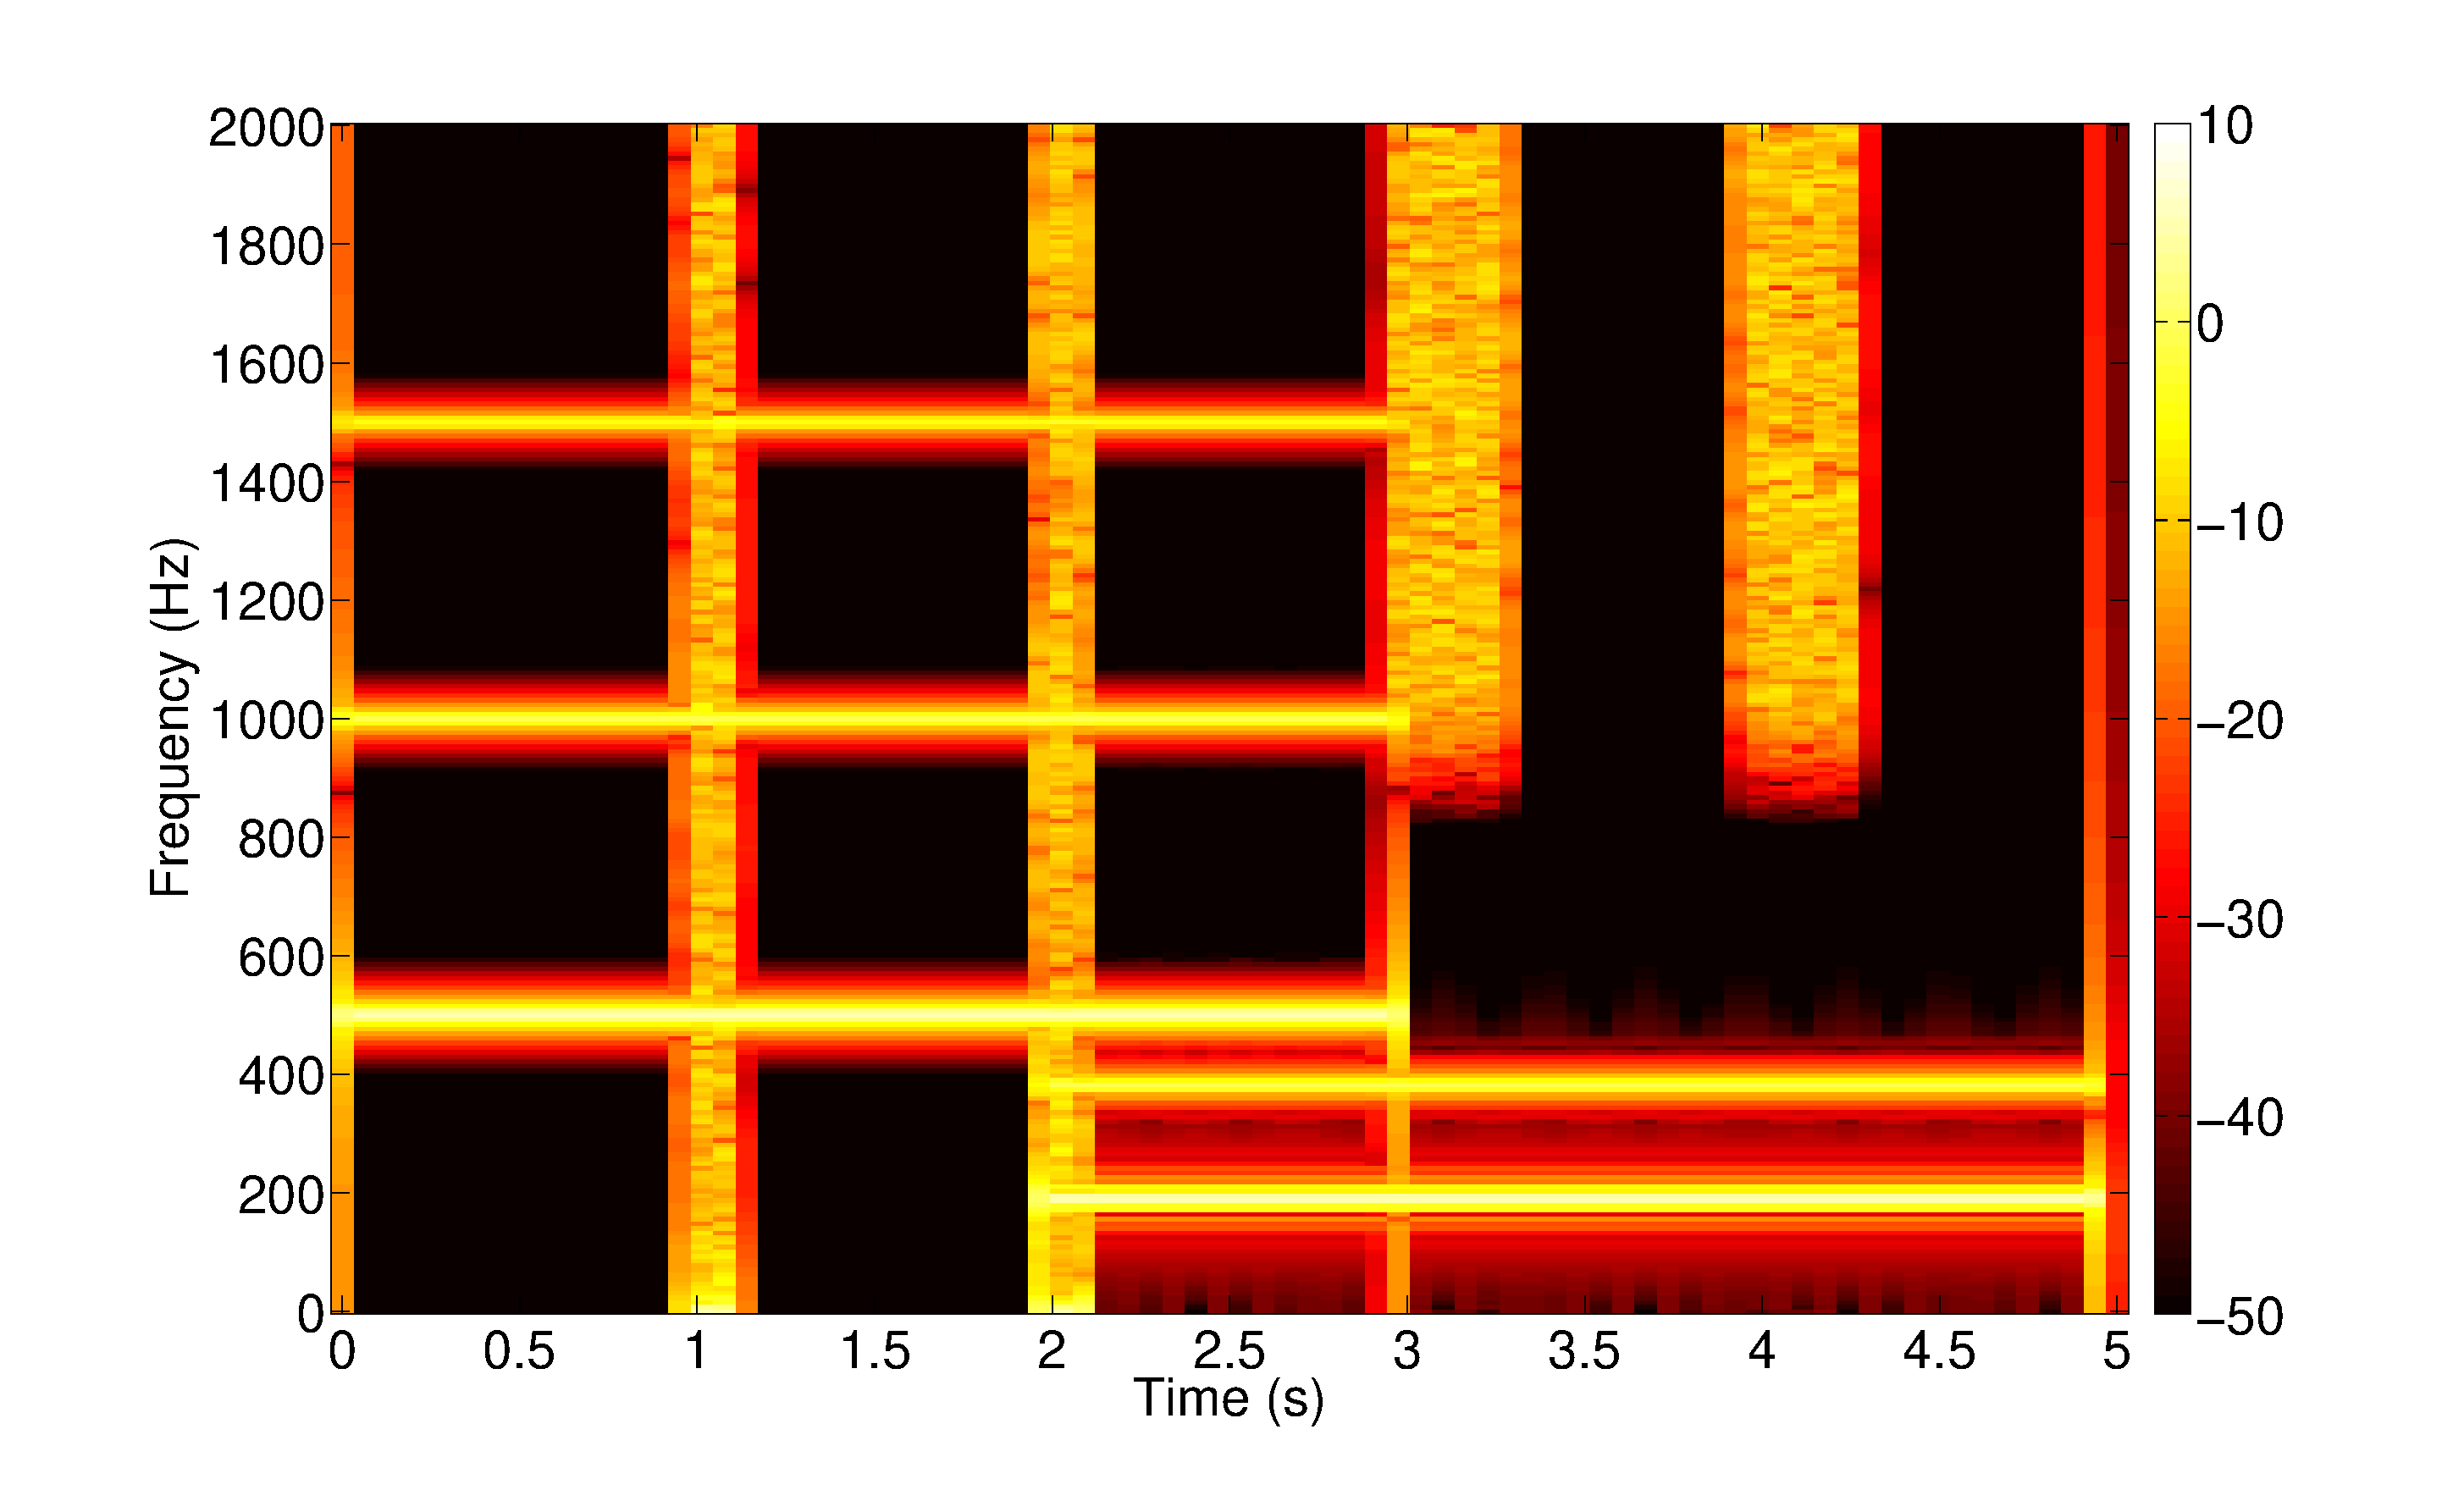
\includegraphics[width=9cm]{fig/synthetictestspectrogram}
%  \vspace{2.0cm}
  \caption{\label{SpectroSynth} Spectrogram of the synthetic test signals.}
  
\end{figure}

\begin{figure*}
   
	\centering    
  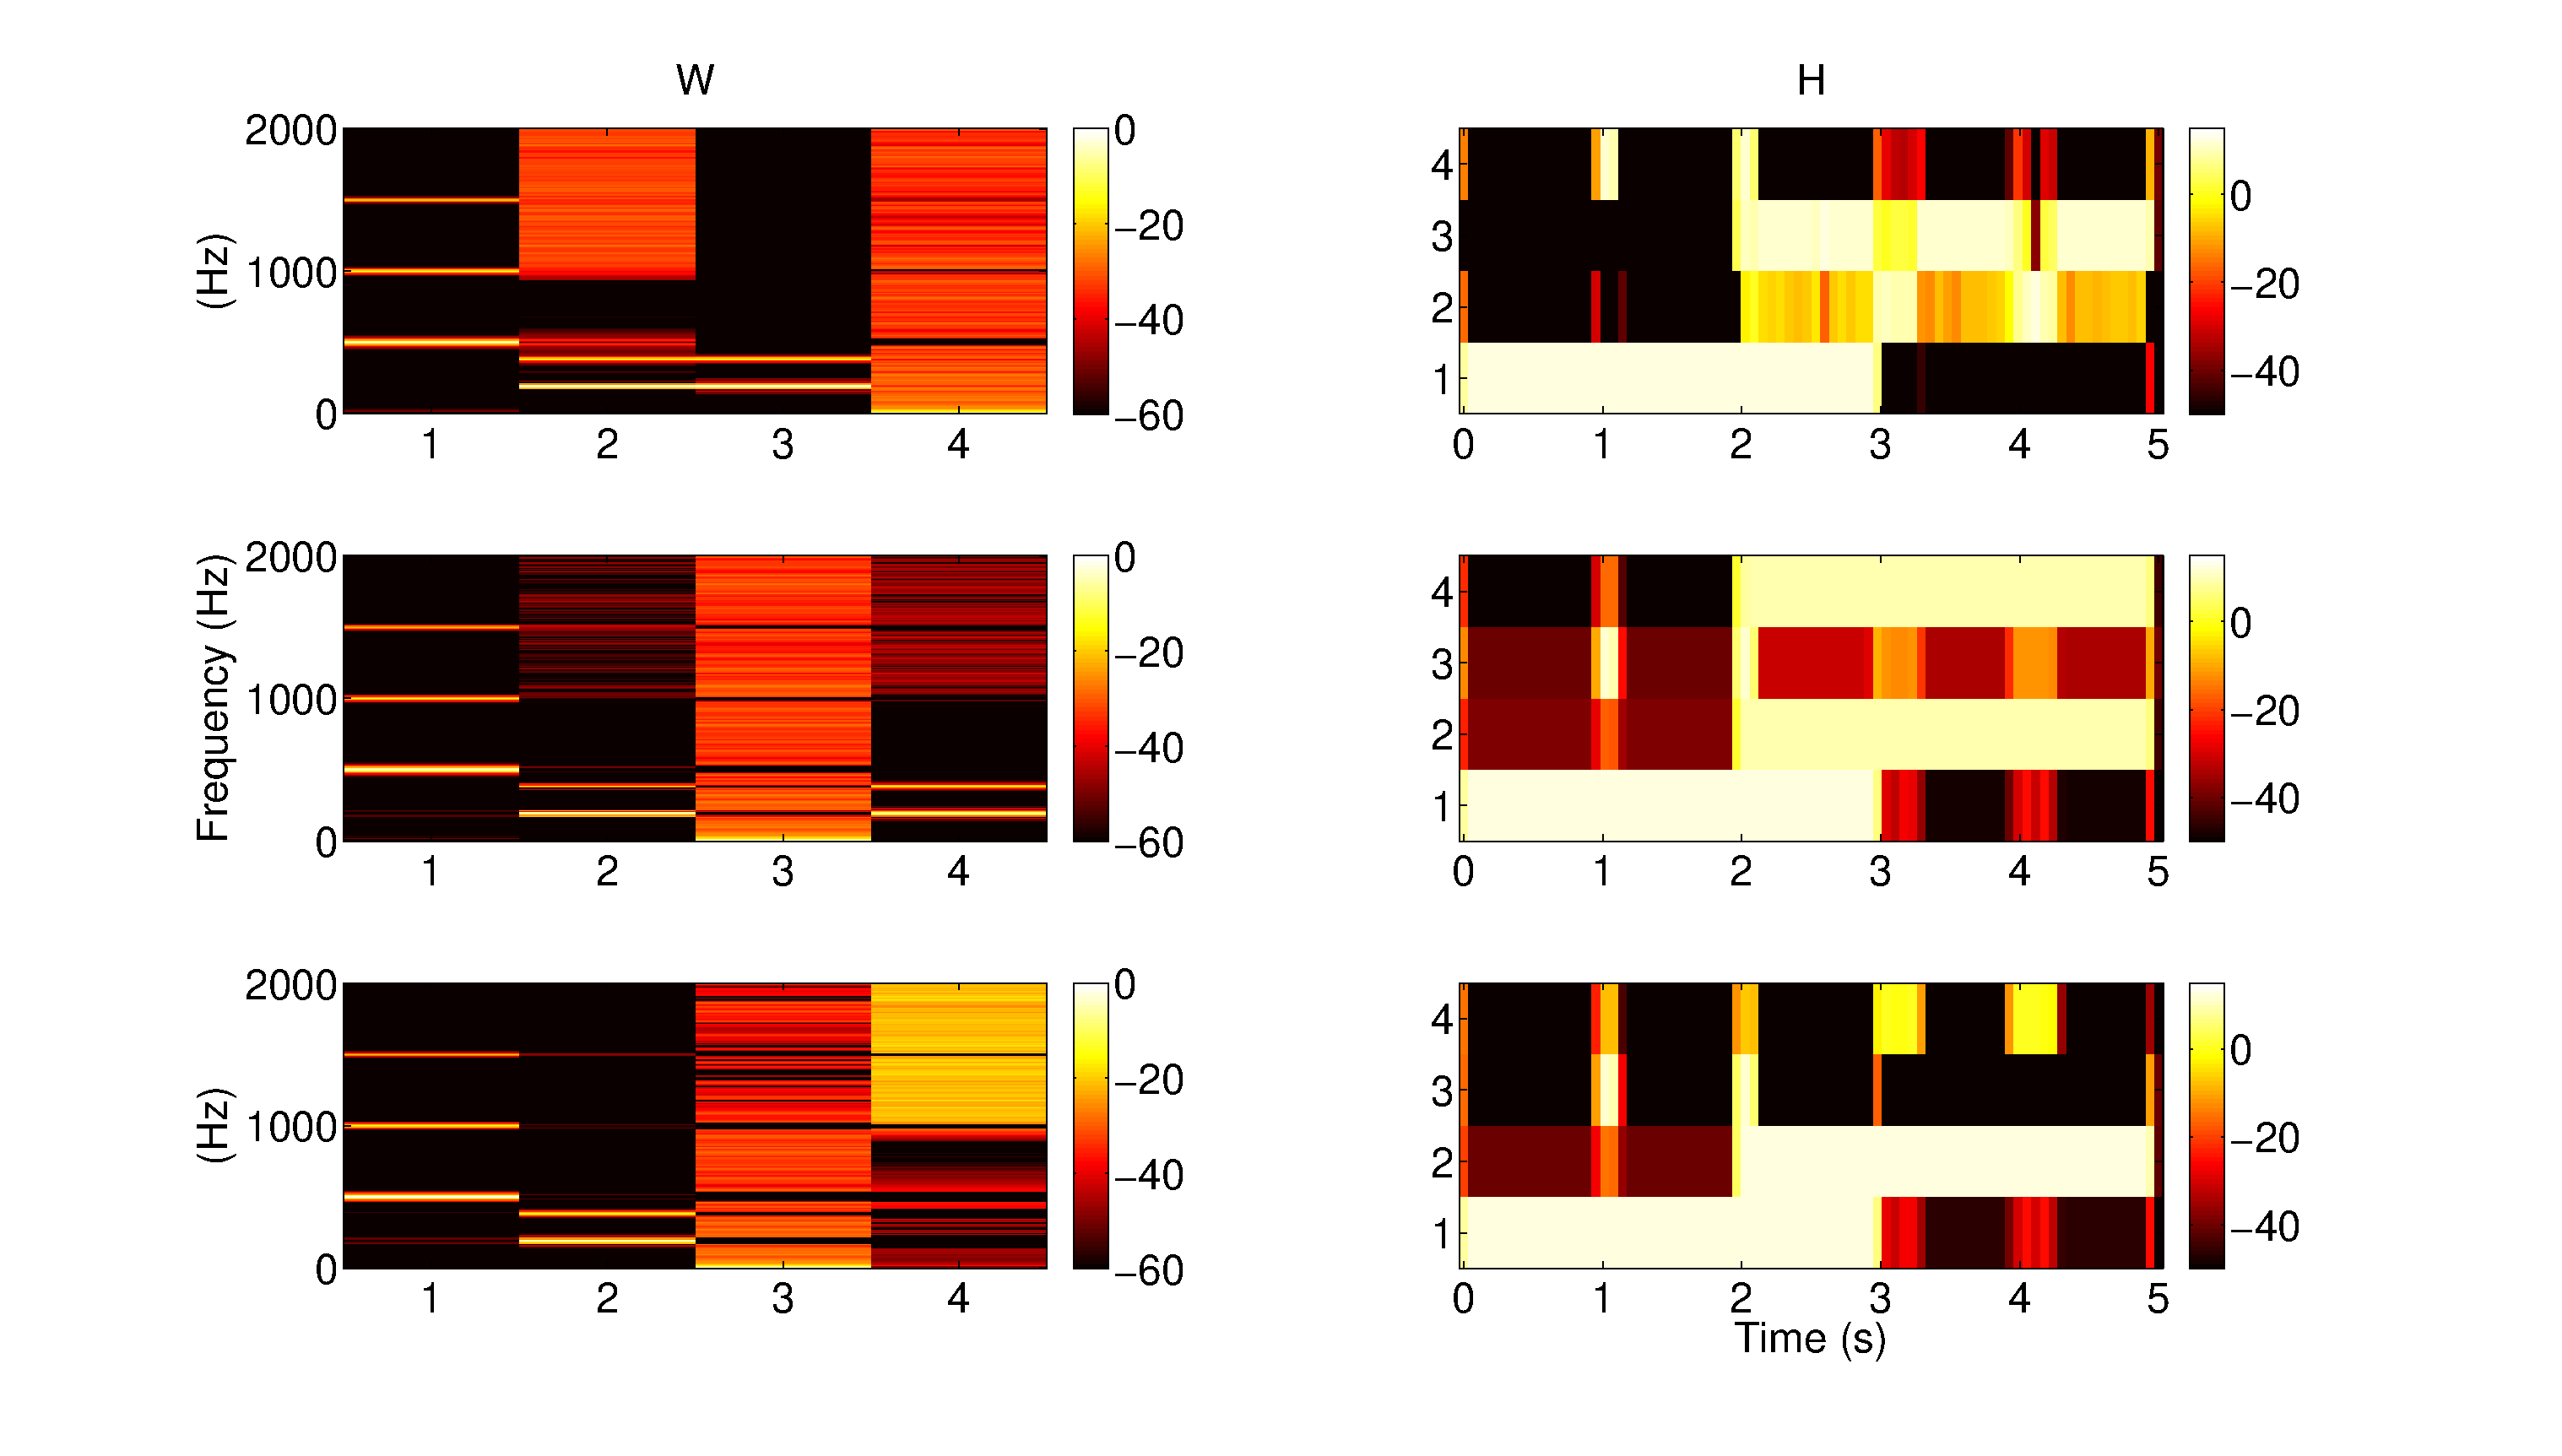
\includegraphics[width=15cm]{fig/WHcomp}

\caption{\label{resultONMF2} Results of the decomposition of the NMF (top matrices), PNMF (middle matrices) and SPNMF (bottom matrices).}


\end{figure*}


\subsection{Protocol and details of the test database}


To understand the behaviour of the SPNMF with the fixed dictionary (Algorithm~\ref{AlgoDictionary}), we run different tests on the public SiSec database from~\cite{SiSec10}. It is composed of polyphonic real-world music excerpts. Each music signal contains percussive, harmonic instruments and vocals. It consists of four recordings whose durations range from $14$ to $24$~s. The goal is to perform a harmonic/percussive decomposition. Following~\cite{canadas2014percussive}, we will not consider the vocal part and we will build mixture signals only from the percussive and harmonic instruments. All the signals are sampled at $44.1kHz$. We compute the STFT with a $1024$ and $2048$ sample-long Hann window with a $50\%$ overlap.
Three tests are run on these data:
\begin{enumerate}
	\item The first test aims at assessing the robustness of the SPNMF with respect to the rank of the PNMF part. 
	\item The second test is to evaluate which of the three divergences (Euc, KL and IS respectively) give the best harmonic/percussive decomposition.
	\item The last test shows the influence of the dictionary on the separation performance. 
\end{enumerate} 
We are using a different database to set-up the proposed method from the one in the evaluation phase in order to prevent any possible over-training and therefore to get the most accurate and fair comparison. 
In order to evaluate and compare the results we then compute the common Signal to Distortion Ratio/Signal to Interference Ration/Signal to Artefact Ratio (SDR/SIR/SAR) metrics for blind source separation with the BSS-Eval toolbox~\cite{bsseval}. 


\subsection{Robustness wrt the rank of the harmonic part}
\label{setup:rank}

In the case where we use a dictionary matrix, the only parameter of the algorithm is the rank of factorization of the harmonic part. We used the SPNMF algorithm with the fixed dictionary obtained from the STFT of a drum signal as described in Section~\ref{fixedict}. The algorithms are implemented using the multiplicative update rules from~\ref{euclidisteq},~\ref{KLdisteq} and~\ref{ISdisteq} and they all are  initialized with the same random non-negative matrices. 
We display the mean value of the separation results on Figure~\ref{RankOfFact}. When the rank of factorization is small, the Euclidean distance and the KL divergence do not obtain satisfying results. However, for $r>=100$, the results for both distances remain stable. With the IS divergence, the results seem independent of the size of the factorization.

The optimization process of SPNMF is straightforward thanks to the robustness of the method wrt the rank of factorization. The number of components that can be decomposed by orthogonal basis functions is limited, and increasing the rank of factorization does not perturb the results as the harmonic part has to be orthogonal. For the rest of the article, the rank of factorization will be set to $r=100$ for all methods.



\begin{figure}[htb]

  \centering 
  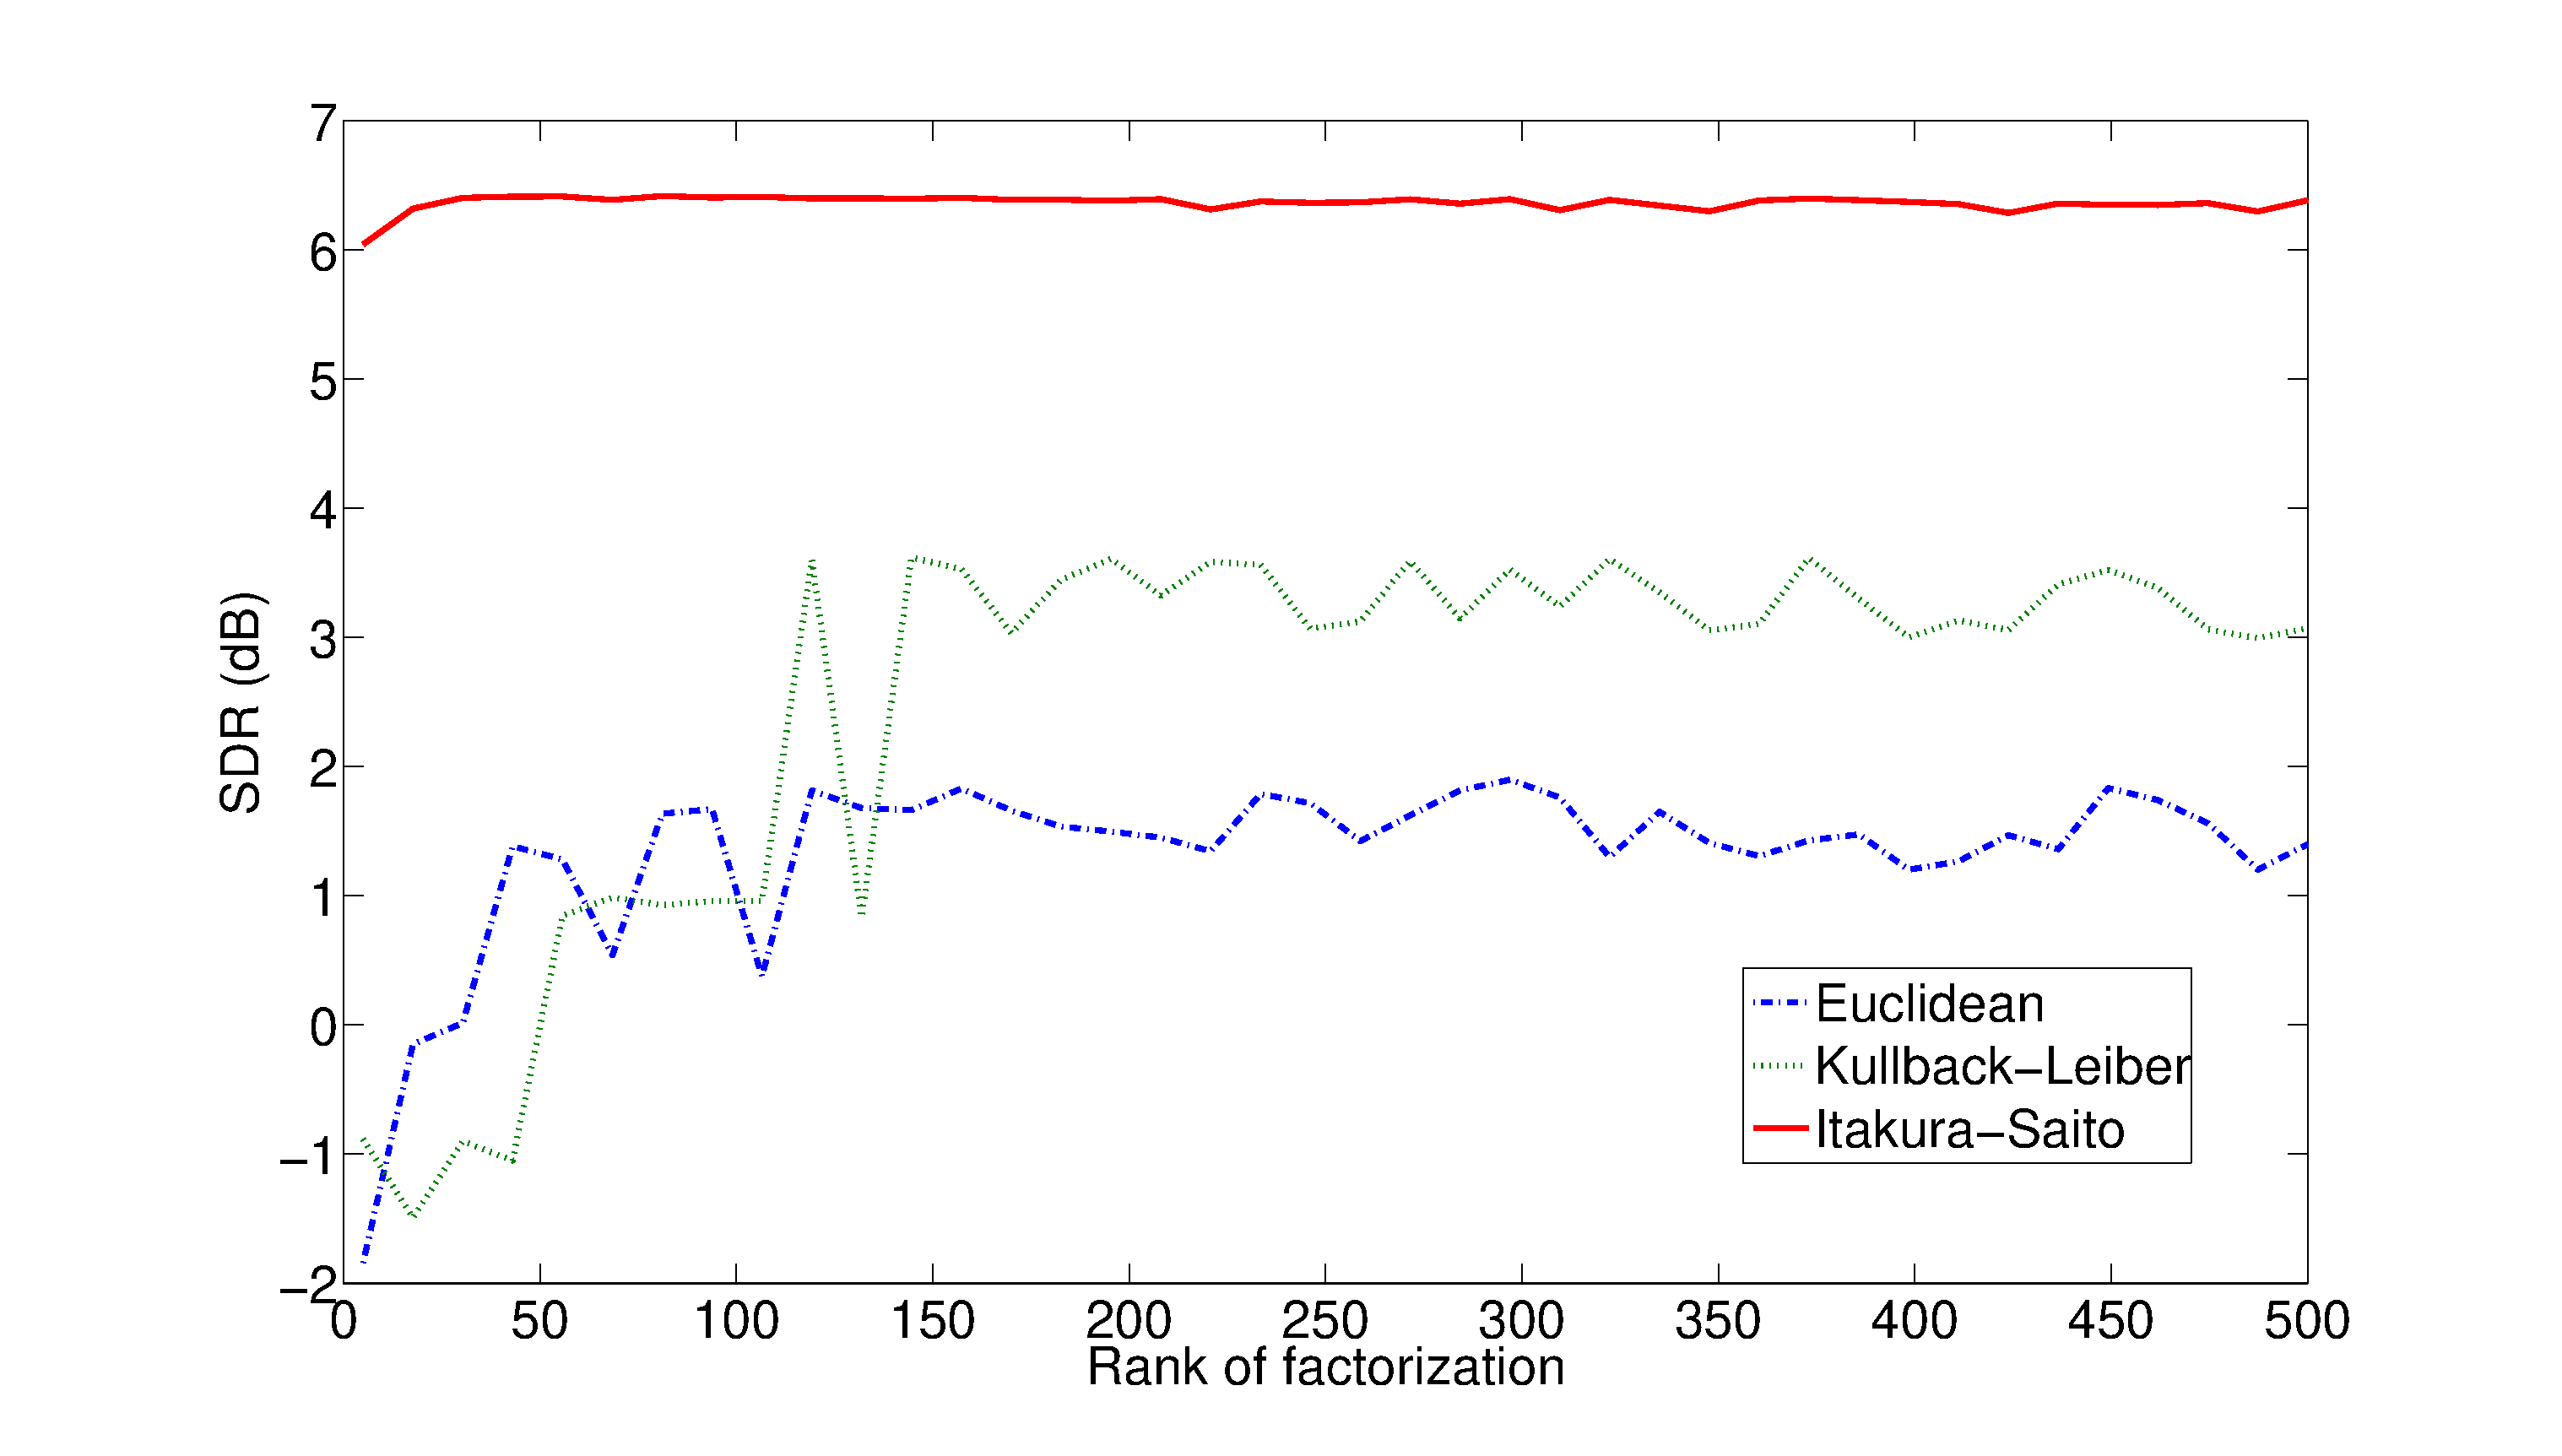
\includegraphics[width=9cm]{fig/RankOfFact}
%  \vspace{2.0cm}
  \caption{\label{RankOfFact} Optimization of the rank of factorization with the three divergences.}
  
\end{figure}




\subsection{Influence of the divergence}
\label{setup:divergence}

In this section we discuss the influence of the divergence in the results of the SPNMF algorithm. It has been established that the IS divergence is well suited for audio signal decomposition~\cite{gray1980distortion}, even if it does not always lead to superior separation performance~\cite{canadas2014percussive}. In this section, we perform a test of the three divergences on the SiSec database to evaluate the performance of the three algorithms. We tried two different window lengths ($1024$ samples and $2048$ samples) for the Fourier transform as it showed interesting results. We display on Figures~\ref{frame1024} and~\ref{frame2048} the mean of the results of the three algorithms on the SiSec database. Each box-plot is made up of a central line indicating the median of the data, upper and lower box edges indicating the $1^{st}$ and $3^{rd}$ quartiles while the whiskers indicate the minimum and maximum values. 

When the frame length is small, the percussive instruments are well represented and the energy is localized. Using a longer window spreads the percussive energy while the tonal components are well separated in the TF domain.

When the frame size is small, Figure~\ref{frame1024} shows that the percussive decomposition is better for the Euclidean distance and the KL divergences. However, the harmonic components are not well separated in the TF domain and the orthogonal part of SPNMF does not perform a good separation.  
In the case of a long window, the Figure~\ref{frame2048} shows that the IS divergence works better than the other divergences. The orthogonal part is more effective to extract the harmonic components as the finer frequency resolution allows for a better separation in the TF domain. The IS divergence is scale invariant. It means that the low energy components of the spectrogram bear the same relative importance as the higher ones which allows a good extraction of the percussive instruments even if the energy is spread temporally.


For the rest of the article, we will use the SPNMF algorithm with the IS divergence and a $2048$ window size in the STFT.


\begin{figure}[htb]

  \centering 
  \includegraphics[width=9cm]{fig/DivergenceFrame1024}
%  \vspace{2.0cm}
  \caption{\label{frame1024} SDR, SIR and SAR of harmonic (left bar)/percussive (right bar) estimated sources on the SiSec database with a window frame of $1024$ samples.}
  
\end{figure}


\begin{figure}[htb]

  \centering 
  \includegraphics[width=9cm]{fig/DivergenceFrame2048}
%  \vspace{2.0cm}
  \caption{\label{frame2048} SDR, SIR and SAR of harmonic (left bar)/percussive (right bar) estimated sources on the SiSec database with a window frame of $2048$ samples.}
  
\end{figure}



\subsection{Influence of the dictionary}
\label{setup:dictionary}

We now discuss the influence of the dictionary. We tried the two methods described in Section~\ref{fixedict} and a third dictionary is made by the concatenation of the two dictionaries. The more information contained in the dictionary, the more there is chance for the decomposition to properly extract the percussive part. On some signals, the decomposition is not able to extract a lot of energy from the mixture as no atom from the dictionary correspond to any of the percussive signal.
We display on Figure~\ref{resultsDict} the SDR results of the decomposition using the NMF dictionary, the STFT dictionary as well as the concatenated dictionary. The SAR and SIR are postponed in Appendix~\ref{appendix:dict} on Figures~\ref{resultsDictSAR} and~\ref{resultsDictSIR} respectively. On our tests, the results with the concatenated dictionary show the highest score. Indeed, the concatenated dictionary contains the largest amount of information and as a result, obtains the best separation. As the dictionary is fixed, it is important to have a large dictionary to extract a large type of percussive instruments. On the other hand, the STFT and the NMF dictionaries obtain similar results. Each dictionary contain complementary informations that allow for a better separation while they are concatenated. For the tests we will conduct later in Section~\ref{sec:stateoftheart} on a large database, we will use the concatenated dictionary as it contains the largest amount of information. 


\begin{figure}[htb]

  \centering 
  \includegraphics[width=8cm]{fig/DictSDR}
%  \vspace{2.0cm}
  \caption{\label{resultsDict} SDR of harmonic (left bar)/percussive (right bar) estimated sources on the SiSec database with a STFT dictionary, a NMF dictionary and the concatenation of the two.}
  
\end{figure}


%\begin{table}
%   
%	\centering    
%   \begin{tabular}{|l|l|l|l|l|}
%  \hline
%  &    & Percussive separation & Harmonic separation  \\
%  \hline
%       & NMF          & 10.28 & 2.69  \\
%  SDR  & STFT         & 10.17 & 2.59  \\
%  (dB) & Concatenated & 10.21 & 2.51  \\  
%  \hline
%       & NMF           & 20.97 & 2.45  \\
%  SIR  & STFT          & 21.11 & 2.61  \\
%  (dB) & Concatenated  & 20.70 & 2.65  \\  
%   \hline
%       & NMF           & 10.70 & 29.41  \\
%  SAR  & STFT          & 10.58 & 29.59  \\
%  (dB) & Concatenated  & 10.65 & 29.58  \\ 
%  \hline
%\end{tabular} 
%\caption{\label{resultsDict} Source separation performance using three dictionaries.}
%
%
%\end{table}
%\vspace{-0.4cm}
%



\section{State of the art Benchmark}
\label{sec:stateoftheart}

In this section, we compare the proposed method with three state of the art methods on a large evaluation database. We detail first the database used and the other state of the art method in Section~\ref{database} and~\ref{soth} respectively.  


\subsection{Database}
\label{database}

The dataset is taken from medley-dB~\cite{bittner2014medleydb} and is composed of polyphonic real-world music excerpts. It has $122$ music signals and $89$ of them contain percussive instruments, harmonic instruments and vocals. The signals that do not contain a percussive part are excluded of the evaluation. The goal is to perform an harmonic/percussive decomposition as in~\cite{canadas2014percussive} thus the vocal part is omitted. All the signals are sampled at $44.1kHz$.

\subsection{State of the art methods}
\label{soth}

We compare here the SPNMF with the dictionary matrix with other recent state of the art methods: constrained NMF~\cite{canadas2014percussive}, HPSS~\cite{fitzgerald2010harmonic} and NMPCF~\cite{kim2011nonnegative}. Constrained NMF and NMPCF are re-implemented in this paper and the HPSS implementation is taken from~\cite{DriedgerMueller14_TSMToolbox_DAFX}.

HPSS is a state of the art, versatile and computationally efficient method. It is widely used in the Music Information Retrieval community and is a good baseline for comparison. The constrained NMF algorithm is the most recent method of harmonic/percussive separation. It gives good results on a small scale test, however the robustness of the algorithm has not been tested yet in a large scale experiment. Finally the NMPCF, similarly to our method, uses a drum dictionary to guide the percussive estimation but the harmonic part is totally unconstrained. 


\subsection{Results} 
\label{subResults}

Figures~\ref{DatabaseSDR},~\ref{DatabaseSIR} and~\ref{DatabaseSAR} show the SDR, SIR and SAR results of the four methods on the selected $89$ songs of the original Medley-dB database~\cite{bittner2014medleydb}. The results on the entire database show that the four methods extract the harmonic instruments much better than the percussive instruments. All methods rely on Wiener filtering for phase reconstruction (see equation~\ref{percuweiner}). As the percussive instruments have flat spectra, the percussive mask is a non sparse matrix and small estimation errors drastically decrease the results of the percussive instruments. This tendency is not visible on small scale tests as it is not always the case (see table~\ref{resultsDict}). 
Figure~\ref{DatabaseSDR} shows that SPNMF obtains on average the highest separation score for the percussive, harmonic and mean SDR. However, the variance of the results of SPNMF is higher than for the other algorithms. Some songs of the database contain percussive instruments that are not present in the learning database ENST-Drums, for example tambourine, bongo, gong and electronic drums. Because the dictionary is fixed, the percussive instruments are not correctly decomposed by the SPNMF. It induces an increase of the variance as some songs are well separated while other obtain much lower results as the percussive part is not well decomposed.

The NMPCF, also based on trained data, is more robust than SPNMF because the dictionary that extract the drums is not fixed. It allows more freedom and the results are more consistent even if some percussive instruments are not in the learning database. However, the mean score is lower than the SPNMF.

The HPSS results obtained in our tests are unsatisfying. A wide variety of harmonic instruments in the database have really strong transients and rich harmonic spectra (distorted electric guitar, glockenspiel,\ldots), similarly, some percussive instruments have sparse basis functions localized in the low frequency range (bass drum, bongo, toms,\ldots). Because of that, HPSS fails to extract these instruments in the appropriate harmonic/percussive parts. On average, it is able to correctly separate the percussive part (with relatively high SDR and the highest SIR) but with a very low SAR compared to the other methods. Similar outcomes have been observed in~\cite{canadas2014percussive} for HPSS.

Similarly, the constrained NMF algorithm relies on the same hypothesis as HPSS and the results are lower than those of SPNMF. Some transients of the harmonic instruments are decomposed in the percussive part, and some percussive instruments (mainly in the low frequency range) are decomposed by the harmonic part. The method is still competitive in the large scale test. 

Compared to the other state of the art methods, SPNMF obtains the higher average results on the selected database. 


\begin{figure}[h]

  \centering 
  \includegraphics[width=9cm]{fig/DatabaseSDR.png}
%  \vspace{2.0cm}
  \caption{\label{DatabaseSDR} SDR for percussive/left, harmonic/middle, mean/right separation results on the database for the four methods.}
  
\end{figure}

\begin{figure}[h]

  \centering 
  \includegraphics[width=9cm]{fig/DatabaseSIR.png}
%  \vspace{2.0cm}
  \caption{\label{DatabaseSIR} SIR for percussive/left, harmonic/middle, mean/right separation results on the database for the four methods.}
  
\end{figure}

\begin{figure}[h]

  \centering 
  \includegraphics[width=9cm]{fig/DatabaseSAR.png}
%  \vspace{2.0cm}
  \caption{\label{DatabaseSAR} SAR for percussive/left, harmonic/middle, mean/right separation results on the database for the four methods.}
  
\end{figure}




\subsection{Results on a genre specific database}
\label{sec:subdata}

The individual results on most of the songs of the database are similar to the average results. However, some interesting results were found on specific genre of music. Here we present the results obtained on $14$ songs of "Electronic/Fusion". These songs for the most part have a lot of silence and some solo parts where only one instrument is playing. Finally on some songs, the electronic drum reproduces the same pattern for the whole song so the drum part is very redundant. The SDR results on the sub-database are displayed on Figure~\ref{ElectroFusionSDR} while the SIR and SAR results are postponed in Appendix~\ref{appendix:sub_database} on Figures~\ref{ElectroFusionSIR} and~\ref{ElectroFusionSAR} respectively. 


The HPSS method gives competitive results, with a low variance for the percussive results and good overall mean. The HPSS obtains consistent results throughout the database. The results on the genre specific database are significantly better than on the whole database. It traduces the fact that the harmonic/percussive instruments are easier to separate on these songs. 
 
The results of NMPCF are the lowest of the four methods. The Unconstrained harmonic part gives the NMPCF a higher degree of freedom that decreases the score as the information is unequally distributed in the harmonic and percussive layer depending on the signal to decompose. 

Finally constrained NMF does not obtain satisfying results on this sub-database. The hyper-parameters are set to the optimal values obtained on a training database of another genre. Because of that, the value of the parameters are not set correctly and similarly to NMPCF, the information is not distributed in the appropriate harmonic/percussive parts. 


On this sub-database, SPNMF outperforms considerably the other methods. Similarly to Section~\ref{subResults}, the percussive decomposition of SPNMF has high variance because some of the instruments are not in the learning database. However, the mean of the percussive decomposition is significantly higher than constrained NMF and NMPCF also the harmonic decomposition and the mean results of SPNMF are clearly above all the other methods. SPNMF is effective to extract the redundant drum parts. Also as the drum dictionary is fixed, it is unlikely for the percussive part to extract harmonic components, similarly, as the columns of $W$ are orthogonal, it is unlikely for the harmonic part to extract percussive components. Contrary to other algorithms, when the harmonic or percussive instruments are playing alone, the SPNMF does not extract any information in the percussive or harmonic part respectively.



\begin{figure}[htb]

  \centering 
  \includegraphics[width=9cm]{fig/ElectroFusionSDR.png}
%  \vspace{2.0cm}
  \caption{\label{ElectroFusionSDR} SDR for percussive/left, harmonic/middle, mean/right separation results on the Electronic/Fusion songs for the four methods.}
  
\end{figure}

\subsection{Discussion}
\label{discu}

The results on the entire database give us insightful information.
HPSS and constrained NMF use the hypothesis that harmonic instruments have sparse tonal spectrogram and percussive instruments have flat transient spectra. They utilize two different methods to extract the instruments (complementary median filtering, and constraints on the NMF decomposition).
NMPCF uses prior learning to extract the percussive instruments in a specific part while the harmonic instruments are decomposed in an unconstrained layer. 
Finally, SPNMF uses both techniques from the previous state of the art methods. It uses prior learning to extract the percussive instruments while the harmonic parts are extracted by the sparse PNMF components.



Each methods have their advantages and  drawbacks. HPSS is the easiest method to implement, the fastest and it does not require any hyper-parameter tuning. The results of HPSS can be competitive when the harmonic instruments have smooth transients (i.e., sustained instruments as flute, violin) and the percussive instruments have flat spectra (i.e., cymbal, snare drum). However, when the harmonic instruments have strong transients (glockenspiel, piano) and the percussive instruments have sparse spectra (bass drum, bongo) the HPSS does not obtain good results. 

The constrained NMF is based on the same hypothesis than HPSS and has the same problem. Fine tuning of the hyper-parameters can alleviate the problem mentioned above but it is a tedious process and is not possible in the case of blind source separation. Our tests on a large database show that the constrained NMF is not robust to a wide variability of the analyzed signals.

Contrary to the results from~\cite{canadas2014percussive} the NMPCF algorithm gives competitive results compare to HPSS and constrained NMF. As it uses training to guide the decomposition process, it requires a wide variety of information to perform on a large scale test. If the training database does not contain sufficient information, the results will not be satisfying. 

On the large scale test, SPNMF outperforms the other methods. It is able to extract the harmonic and the percussive instruments with higher score for SDR, SAR and SIR. Using prior dictionary learning with a physical model on the harmonic instruments help to separate the instruments with much better accuracy.

In our test, the training database of SPNMF and NMPCF is only composed of drum sounds, however the database~\cite{bittner2014medleydb} contains a wide variety of percussive instruments that are not in the training database. We decided not to include these types of percussion in the training database as we wanted to have a comparable computation time between the four methods and to test the robustness of the supervised methods when a percussive signal is not in the database. 



\section{Conclusion}
\label{sec:conc}

In this article, we demonstrate that SPNMF is a very promising model for harmonic/percussive decomposition. Indeed, the SPNMF outperforms three other state of the methods on the medley-dB database~\cite{bittner2014medleydb}. Carrying out an evaluation on a large database allowed us to compare more accurately the performance of the four methods on a large variety of music signals. 

On a large database none of the state of the art methods produces a satisfying harmonic/percussive source separation. The large variety of audio signal makes the task extremely difficult. That said, on a smaller section of the database, the SPNMF showed some promising results (see~\ref{sec:subdata}).

We can say that the information from the drum dictionary built from the database ENST-Drums~\cite{gillet2006enst} is not sufficient to perform a harmonic/percussive source separation on a large scale. Depending of the style of music, some drums share similarities. A possible improvement would be to build genre specific drum dictionaries. In this way, the computation time would be reasonable as the amount information could be reduced and the templates of the dictionary could be a lot more focused on specific type of drums. 





\section*{Annexe}

\subsection{Euclidean distance}
\label{euclidisteq}

The euclidean distance gives us the problem,
$$\min_{W_1,W_2,H_2 \geq 0} \|V - W_{1}W_{1}^{T}V + W_{2} H_{2} \|^2.$$
The gradient wrt $W_1$ gives the update
$$[\nabla_{W_1} D(V|\tilde{V})]^{-} = 2 VV^TW_1, $$
and
\begin{align*}
[\nabla_{W_1} D(V|\tilde{V})]^{+} = 2VH_2^TW_2^TW_1 + W_2H_2V^TW_1 + \\ VV^TW_1W_1^TW_1 + W_1W_1^TVV^TW_1.
\end{align*}

Similarly, the gradient wrt $W_2$ gives
$$ [\nabla_{W_2} D(V|\tilde{V})]^{-} = VH_2^T $$
and
$$ [\nabla_{W_2} D(V|\tilde{V})]^{+} = 2W_1W_1^TVH_2^T + W_2H_2H_2^T.$$

Finally, the gradient wrt $H_2$ gives
$$ [\nabla_{H_2} D(V|\tilde{V})]^{-} = W_2^TV  $$
and
$$ [\nabla_{H_2} D(V|\tilde{V})]^{+} = 2W_2^TW_1W_1^TV + W_2^TW_2H_2. $$


\subsection{Kullback Leiber divergence}\label{KLdisteq}
The Kullback Leiber divergence gives us the problem,
$$\min_{W_1,W_2,H_2 \geq 0} V(log(V) - log(\tilde{V})) + (V-\tilde{V}).$$

The gradient wrt $W_1$ gives
$$[\nabla_{W_1} D(V|\tilde{V})]_{i,j}^{-} = (ZV^TW_1)_{i,j} + (VZ^TW_1)_{i,j},$$
with $Z_{i,j} = (\frac{V}{W_1W_1^TV + W_2H_2})_{i,j}$. The positive part of the gradient is
$$[\nabla_{W_1} D(V|\tilde{V})]^{+}_{i,j} = \sum_k(W^TV)_{j,k} + (\sum_{k}V_{i,k})(\sum_a W_{a,j}).$$


Similarly, the gradient wrt $W_2$ gives
$$ [\nabla_{W_2} D(V|\tilde{V})]^{-} = VH_2^T $$
and
$$ [\nabla_{W_2} D(V|\tilde{V})]^{+} = W_1W_1^TVH_2^T + W_2H_2H_2^T.$$

Finally, the gradient wrt $H_2$ gives
$$ [\nabla_{H_2} D(V|\tilde{V})]^{-} = W_2^TV  $$
and
$$ [\nabla_{H_2} D(V|\tilde{V})]^{+} = 2W_2^TW_1W_1^TV + W_2^TW_2H_2. $$

 
\subsection{Itakura Saito divergence}\label{ISdisteq}
The Itakura Saito divergence gives us the problem,
$$\min_{W_1,W_2,H_2 \geq 0} \frac{V}{\tilde{V}} - log(\frac{V}{\tilde{V}}) +1.$$

The gradient wrt $W_1$ gives
$$[\nabla_{W_1} D(V|\tilde{V})]_{i,j}^{-} = (ZV^TW_1)_{i,j} + (VZ^TW_1)_{i,j},$$
with $Z_{i,j} = (\frac{V}{W_1W_1^TV + W_2H_2})_{i,j}$. 
The positive part of the gradient is
$$[\nabla_{W_1} D(V|\tilde{V})]_{i,j}^{-} = (\phi V^TW_1)_{i,j} + (V \phi^T W_1)_{i,j},$$
with $$ \phi_{i,j} = (\frac{I}{W_1W_1^TV + W_2H_2})_{i,j}.$$ and $I = ones(size(V))$.


Similarly, the gradient wrt $W_2$ gives
$$ [\nabla_{W_2} D(V|\tilde{V})]^{-} = VH_2^T $$
and
$$ [\nabla_{W_2} D(V|\tilde{V})]^{+} = W_1W_1^TVH_2^T + W_2H_2H_2^T.$$

Finally, the gradient wrt $H_2$ gives
$$ [\nabla_{H_2} D(V|\tilde{V})]^{-} = W_2^TV  $$
and
$$ [\nabla_{H_2} D(V|\tilde{V})]^{+} = 2W_2^TW_1W_1^TV + W_2^TW_2H_2. $$



\subsection{SAR and SIR results with the different dictionaries}
\label{appendix:dict}

\begin{figure}[H]
  \centering 
  \includegraphics[width=8cm]{fig/DictSAR.png}
  \caption{\label{resultsDictSAR} SAR of harmonic (left bar)/percussive (right bar) estimated sources on the SiSec database with a STFT dictionary, a NMF dictionary and their concatenation.}
\end{figure}

\begin{figure}[H]
  \centering 
  \includegraphics[width=8cm]{fig/DictSIR.png}
  \caption{\label{resultsDictSIR} SIR of harmonic (left bar)/percussive (right bar) estimated sources on the SiSec database with a STFT dictionary, a NMF dictionary and their concatenation.}
\end{figure}

\subsection{Results on the sub database}
\label{appendix:sub_database}

\begin{figure}[H]
  \centering 
  \includegraphics[width=9cm]{fig/ElectroFusionSIR.png}
  \caption{\label{ElectroFusionSIR} SIR for percussive/left, harmonic/middle, mean/right separation results on the Electronic/Fusion songs for the four methods.} 
\end{figure}

\begin{figure}[H]
  \centering 
  \includegraphics[width=9cm]{fig/ElectroFusionSAR.png}
  \caption{\label{ElectroFusionSAR} SAR for percussive/left, harmonic/middle, mean/right separation results on the Electronic/Fusion songs for the four methods.}
\end{figure}



\section*{Acknowledgment}




\bibliographystyle{IEEEtran}
% argument is your BibTeX string definitions and bibliography database(s)
\bibliography{reference}


\end{document}
